% !TEX root = ../thesis.tex
\chapter{Grundlagen}\label{chap:grundlagen}
Dieses Kapitel widmet sich den Grundlagen für diese Arbeit. Hierzu gehört die Definition der Modellannahmen.
Des Weiteren werden Optimierungsverfahren vorgestellt. Der Schlussteil des Kapitels widmet sich dem optischen Fluss, durch den Bewegungen geschätzt werden.

\section{Schwarmverhalten}

Die Verhaltensbiologie unterscheidet die Begriffe Verhaltensweisen und Verhaltensmuster.
Ersteres sind voneinander unterscheidbare und beobachtbare Bewegungsabläufe. Das sind beispielsweise Bewegung des Körpers oder Körperhaltung. Das Verhaltensmuster ist durch beobachtbare Abfolgen von Verhaltensweisen definiert.
Schwarmverhalten wird als komplexes Verhaltensmuster definiert \cite{Hamann}

\subsection{Boids}\label{sec:Boids}
\usetikzlibrary{matrix,chains,positioning,decorations.pathreplacing,arrows,shapes,snakes}


Boids ist ein Modell, welches von Reynolds 1987 veröffentlicht wurde. Seine Intention war es, ein Modell zu präsentieren, welches Schwarmverhalten simuliert, um dies für Animationen nutzen zu können. Die Grundvoraussetzungen für einen Schwarm sind das Zusammenhalten der Individuen, eine gemeinsame Bewegungsrichtung und das Vermeiden von zu geringen Abständen zwischen den Individuen. Um dies zu erreichen, setzt Reynolds auf ein agentenbasiertes Modell, d.h.jeder Agent im Schwarm handelt individuell. Der Schwarm wird dadurch zu einer Einheit, die sich selbst organisieren kann, ohne durch eine zentrale Stelle gesteuert zu werden. Ursprünglich formulierte Reynolds für seine Agenten drei zentrale Theoreme.


\begin{figure}[h]
\centering
\begin{tabular}{ccc}
\includegraphics[width=40mm]{figures/Grundlagen/separation.png} &
\includegraphics[width=40mm]{figures/Grundlagen/alignment.png} &
\includegraphics[width=40mm]{figures/Grundlagen/cohesion.png} \\
(a) & (b) & (c)\\
\end{tabular}
\caption{Verhaltensmuster nach Reynolds, \label{fig:BoidsRegeln} entnommen aus \citep{Reynolds1999}}
\end{figure}

a ) \textbf{Abstandsregel} \\
Jeder Agent versucht das Zusammenstoßen mit anderen Agenten zu vermeiden. Hierbei betrachtet der Agent alle Agenten in einem bestimmten Radius R. 
In Abbildung \ref{fig:BoidsRegeln} (a) ist zu sehen wie sich der Agent in Grün von den anderen Agenten innerhalb der Zone wegbewegt. Dies hat zur Folge, dass die Dichte des Schwarms nicht zu groß wird.

b ) \textbf{Angleichen}\\
Der Agent möchte in die gleiche Richtung schwimmen wie Agenten in einer definierten Zone.
Dadurch agiert das Kollektiv als eine Einheit und bewegt sich in dieselbe Richtung.

c ) \textbf{Zusammenbleiben}\\
Der Agent hat das Ziel, beim Schwarm zu bleiben. Dazu schwimmt er in Richtung des Massezentrums welches durch die Agenten in der Zone entsteht.

Zu beachten ist, dass Reynolds in seinem Paper nur die Idee für ein Modell gibt. Ein expliziter Algorithmus wird jedoch nicht definiert \citet{reynolds1987}.


Das Modell nach Reynolds ist rein metrisch, jedoch hat eine Studie von Ballerini \citet{Ballerini} gezeigt, dass insbesondere Stare nur die sechs bis sieben nächsten Nachbarn, unabhängig von deren Distanz wahrnehmen.
Dies wird als topologischer Ansatz bezeichnet.

\begin{figure}[h]
\centering
\includegraphics[width=90mm]{figures/Grundlagen/TopologischVSMetrisch.png}
\caption{Metrisch und Topoligische Distanzen, \label{fig:Dist} entnommen aus \citep{Hamann}}
\end{figure}

Insofern kann das Modell von Reynolds auch durch den topologischen Ansatz formuliert werden.
Hierbei werden die drei Zonen auf die $n$-nächsten Nachbarn aufgeteilt. Der Vorteil an diesem Modell ist, dass der Kontakt zum Schwarm nie verloren geht. Beim metrischen Modell ist es möglich, dass sich ein Agent von dem Schwarm so weit entfernt, dass kein Kontakt mehr zu anderen Agenten besteht. Das topologische Modell hingegen gewährleistet stets eine Verbindung zum Kollektiv. Das eben beschriebene Szenario tritt hauptsächlich bei plötzlichen externen Ereignissen auf. Beispielsweiße ist ein Angriff auf ein Kollektiv so ein Szenario, bei dem einzelne Agenten vom Schwarm getrennt werden. Individuen im Schwarm gelten jedoch als stärker, als solche die sich vom Schwarm getrennt haben. Daher ist das Ziel eines Schwarms das Zusammenbleiben, was robuster durch das topologische Modell als durch das metrische Modell erreicht wird.



\section{Kombinatorische Optimierung}


Kombinatorische Optimierung bezeichnet das Auffinden einer oder mehrerer Teilmengen aus einer Grundmenge an Variablen, welche bezüglich einer Kostenfunktion maximal oder minimal sind. Kombinatorische Optimierung ist ein relevantes Forschungsthema und hat durch Machine Learning und auch insbesondere durch künstliche neuronale Netze einen immer größer werdende Relevanz.
\citet{Agarwal2019P.K}

Mathematisch kann man ein Optimierungsproblem bezüglich einer Kostenfunktion folgendermaßen definieren:

Sei $f: \mathbb{R}^D\rightarrow \mathbb{R}$ eine Fehlerfunktion.

Dann wird $\hat{x}$ gesucht, so dass $f(\hat{x}) \geq f(x) \; \; \; \forall x \in \mathbb{R}^D$
\\
Analog für die Suche des Minimums.

\section{Gradientenabstieg}

Der Gradientenabstieg ist eine Methode, um das Minimum oder auch Maximum einer Funktion zu berechnen. Hierbei wird über die Steigung an einer Stelle ermittelt, in welche Richtung die Extremstelle liegt. Wenn kein Vorwissen über die Position 
der Extremstelle besteht, wird die Startposition zufällig gewählt. Von dieser Position aus wird nun die Steigung bestimmt, um sich in Richtung der Extremstelle zu bewegen.


\begin{figure}[H]
\centering
\includegraphics[width=0.8\linewidth]{figures/Grundlagen/valley_with_ball.png} 
\caption{Gradientenabstieg visualisiert \label{fig:GradVisual} entnommen von \url{http://neuralnetworksanddeeplearning.com/chap1.html} besucht am 24.11.2021}
\end{figure}

Abbildung \ref{fig:GradVisual} visualisiert den Gradientenabstieg. Der grüne Ball symbolisiert die Position an der die Steigung berechnet wird. Der Pfeil stellt die Schrittweite des Abstiegs dar. Die Schrittweite welche auch als Lernrate bezeichnet wird, ist ein kritischer Aspekt. Wird diese zu groß gewählt, so oszilliert der Ball um die Extremstelle und erreicht diese eventuell nicht. Ist diese hingegen zu klein, so dauert der Abstieg unverhältnismäßig lange. Ein Verfahren welches dieses Problem löst nennt sich \textit{ADAM} und steht für adaptive moment estimation.
ADAM ist eine Methode um die Lernrate anzupassen und wird häufig als Alternative zum Stochastic Gradient Descent (SGD) im Deep Learning Bereich verwendet.
Die Regel für das Anpassen der Position lautet:

\begin{subequations}
  \begin{align}
m_t &= \beta_1 \cdot m_{t-1} + (1-\beta_1) \cdot g_t \label{eq:Adam_1} \\
n_t &= \beta_2 \cdot n_{t-1} + (1-\beta_2) \cdot g_t^2 \label{eq:Adam_2} \\
\hat{m}_t &= \frac{m_t}{1-\beta_1^t}  \label{eq:Adam_3} \\
\hat{n}_t &= \frac{n_t}{1-\beta_2^t} \label{eq:Adam_4} \\
v_t &= v_{t-1} - \lambda \cdot \frac{\hat{m}_t}{\sqrt{\hat{n_t}+\epsilon}} \label{eq:Adam_5}
\end{align}
\end{subequations}

In Gleichung \ref{eq:Adam_1} und \ref{eq:Adam_2} bezeichnet $g_t$ den berechneten Gradienten an einer gegebenen Stelle. Initialisiert wird $m_0$ und $n_0$ mit $0$. Die Parameter $\beta_1$ und $\beta_2$ werden mit $0.9$ und $0.999$ angegeben. Die Variablen $m_t$ und $n_t$ bringen die vergangenen Gradienten in den Updateprozess mit ein.
Dadurch fallen plötzliche Richtungsänderungen weniger dramatisch aus.
Der Parameter $\epsilon$ ist eine Konstante und wird mit $\epsilon = 10^{-8}$ angegeben.
$\lambda$ ist die Lernrate und $v_t$ die schlussendliche Schrittrichtung \citet{Adam}.



  Zu erwähnen ist, dass beim Gradientenabstieg nicht sichergestellt werden kann, dass das Minimum auch ein globales und nicht nur ein lokales Minimum ist (gleiches gillt für das Maximum).
Ausgenommen hiervon sind konvexe Optimierungsprobleme. Bei dieser Art ist jedes lokale Minimum/Maximum auch ein Globales.

\subsection{Reverse mode differentiation}\label{sec:RMD}

Das Berechnen von Ableitungen hat im Bereich der Optimierung einen sehr hohen Stellenwert.
Für viele Problemstellungen können Ableitungen nicht analytisch berechnet werden, lediglich die Auswertung an bestimmten Stellen ist möglich. Die Ableitung an einer bestimmten Stelle ist essenziell, um den Gradientenabstieg zu ermöglichen.
Für eine differenzierbare Funktion, welche in numerischer Form vorliegt, ist Reverse Mode Differentiation (RMD) ein Verfahren, um deren Ableitung zu berechnen. Grundbaustein hierfür ist die Kettenregel \cite{DBLP:journals/corr/abs-1811-05031}.

Betrachten wir eine Funktion $z = f(f_1(t),f_2(t))$, welche von zwei weiteren Funktionen $f_1$ und $f_2$ abhängt. Die Funktionen $f_1$ und $f_2$ hängen wiederum von $t$ ab. Dafür sieht die Kettenregel hierfür wie folgt aus:

\begin{equation}\label{eq:Kettenregel}
\frac{\delta z}{\delta t} = \frac{\delta z}{\delta f_1}\frac{\delta f_1}{\delta t} + \frac{\delta z}{\delta f_2}\frac{\delta f_2}{\delta t} 
\end{equation}

Dies kann grafisch folgendermaßen dargestellt werden:

\begin{figure}[H]
 \centering
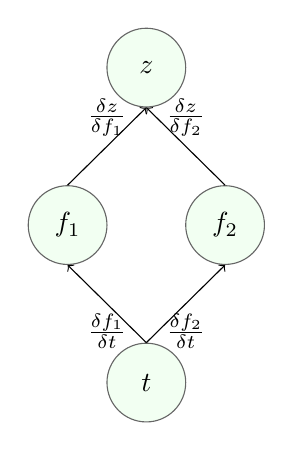
\begin{tikzpicture}[
inputnode/.style={circle, draw=black!60, fill=green!5,  minimum size=10mm},
input/.style={circle},
outputnode/.style={circle},
]
\node[inputnode]          (z)      at (3,2) 		 {$z$};
\node[inputnode]          (x)      at (2,0) 		 {$f_1$};
\node[inputnode]          (y)      at (4,0) 		 {$f_2$};
\node[inputnode]          (t)      at (3,-2) 		 {$t$};

\draw[->] (t.north) -- node[below] {$\frac{\delta f_1}{\delta t}$} (x.south);
\draw[->] (t.north) -- node[below] {$\frac{\delta f_2}{\delta t}$} (y.south);
\draw[->] (x.north) -- node[above] {$\frac{\delta z}{\delta f_1}$} (z.south);
\draw[->] (y.north) -- node[above] {$\frac{\delta z}{\delta f_2}$} (z.south);

\end{tikzpicture}
\caption{Kettenregel als Graph \label{fig:KettenregelGraph}}
\end{figure}

Die grafische Darstellung einer Funktion, wie sie in Abbildung \ref{fig:KettenregelGraph} zusehen ist, kann für jede differenzierbare Funktion angewandt werden. Folgt man dem Graphen ''rückwärts'' von oben nach unten, erhält man Einsicht über die Abhängigkeiten der Ableitung. Es kann also mittels Kettenregel die Ableitung einer Funktion an jeder Stelle berechnet werden. Nachfolgend ist ein Beispiel zu sehen, welches dies veranschaulicht.

Betrachten wir folgende Funktion:

\begin{equation}\label{eq:funktion1}
f(x_1,x_2) = x_1 + x_2 sin(x_1)+ln(x_2)
\end{equation}

Dies lässt sich in komponentenschreibweise ausdrücken, wodurch sich folgender Graph ergibt:

\begin{minipage}{0.4\textwidth}
\begin{subequations}
\begin{align*}
w_0 & = x_1 \\
w_1 & = x_2 \\
w_2 & = w_1 sin(w_0)\\
w_3 & = w_0 + w_2 \\
w_4 & = z = w_3 + ln(w_1)\\
\end{align*}
\end{subequations}
\end{minipage}\hspace{0.1cm}
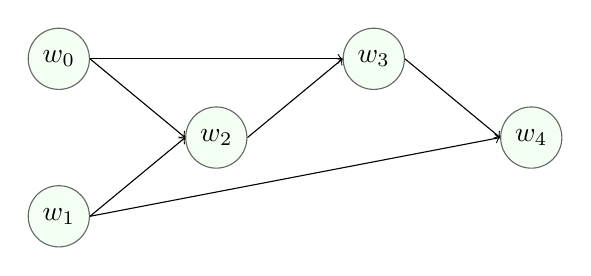
\begin{tikzpicture}[baseline,
inputnode/.style={circle, draw=black!60, fill=green!5,  minimum size=5mm},
input/.style={circle},
outputnode/.style={circle},
]
\node[inputnode]          (w0)      at (2,1) 		 {$w_0$};
\node[inputnode]          (w1)      at (2,-1) 		 {$w_1$};
\node[inputnode]          (w3)      at (4,0) 		 {$w_2$};
\node[inputnode]          (w4)      at (6,1) 		 {$w_3$};
\node[inputnode]          (w5)      at (8,0) 		 {$w_4$};

\draw[->] (w0.east) -- node[below] {} (w3.west);
\draw[->] (w1.east) -- node[below] {} (w3.west);
\draw[->] (w0.east) -- node[below] {} (w4.west);
\draw[->] (w3.east) -- node[below] {} (w4.west);
\draw[->] (w4.east) -- node[below] {} (w5.west);
\draw[->] (w1.east) -- node[below] {} (w5.west);
\end{tikzpicture}


Soll nun die Ableitung an der Position $x_1 = 2, x_2 = 3$ bestimmt werden, so wird der sogenannte \textit{Forwardpass} durchlaufen. Hierbei wird der Graph vom Start bist zum Ende durchlaufen, wobei auf dem Weg die nötigen Ableitungen berechnet werden können.

\begin{subequations}
\begin{align*}
w_0 & = 2 \\
w_1 & = 3 \\
w_2 & = w_1sin(w_0) & \frac{\delta w_2}{\delta w_1} & = sin(w_0) = 0.909 & \frac{\delta w_2}{\delta w_0} &= w_1cos(w_0) & &= -1.24 \\
w_3 & = w_1 + w_2 & \frac{\delta w_3}{\delta w_1} & = 1 & \frac{\delta w_3}{\delta w_2} &= 1 \\
w_4 & = z = w_3 + ln(w_1) & \frac{\delta w_4}{\delta w_3} &= 1 & \frac{\delta w_4}{\delta w_1} &= \frac{1}{w_1} & &=\frac{1}{3}\\
\end{align*}
\end{subequations}


Mit Hilfe der Kettenregel kann nun $\frac{\delta w_4}{\delta w_0}$ und $\frac{\delta w_4}{\delta w_1}$ berechnet werden. Der Graph und der \textit{Forwardpass} geben Aufschluss über die Abhängigkeiten der Ableitungen sowie dessen Werte.
Die Ableitungen werden folgendermaßen berechnet:

\begin{subequations}
\begin{align*}
\frac{\delta w_4}{\delta w_0} & = \frac{\delta w_4}{\delta w_3} \frac{\delta w_3}{\delta w_2}\frac{\delta w_2}{\delta w_0} + \frac{\delta w_4}{\delta w_3} \frac{\delta w_3}{\delta w_0 } &= 1 \cdot 1 -1.24 + 1 \cdot 1 &= -0.24 \\
\frac{\delta w_4}{\delta w_1} & = \frac{\delta w_4}{\delta w_3} \frac{\delta w_3}{\delta w_2} \frac{\delta w_2}{\delta w_1} + \frac{\delta w_4}{\delta w_1} &= 1 \cdot 1 \cdot 0.909 + \frac{1}{3} & = 1.242
\end{align*}
\end{subequations}

Das Rückwärtslaufen auf dem Graphen wird auch als \textit{Backwardpass} bezeichnet.
Das Resultat ist die Ableitung an der Stelle (2,3) und kann für den Gradientenabstieg genutzt werden.


\section{Particle swarm optimisation}\label{sec:PSO}

Particle swarm optimization (PSO) ist ein Verfahren, um optimale Parameter eines Optimierungsproblems zu finden. Es wurde 1995 von Russell C. Eberhart und James Kennedy publiziert. Der Algorithmus wird als Metaheuristik eingestuft, d.h. es ist nicht garantiert, dass eine optimale Lösung gefunden wird.
Prinzipiell kann jedoch eine Lösung gefunden werden. Während beim Gradientenabstieg die Steigung der Kostenfunktion entscheidend ist, kommt PSO ganz ohne Ableitung der Kostenfunktion aus. Der Vorteil ist, dass das Optimum einer nicht ableitbaren Funktion bestimmt werden kann.

Wie der Name PSO vermuten lässt, handelt es sich um einen Algorithmus, der auf Schwarmverhalten setzt. Jeder einzelne Agent wird als Partikel bezeichnet, dessen Position im D-dimensionalen Raum eine potenzielle Lösung des Optimierungsproblems darstellt.
Die Partikel tasten den Raum Schritt für Schritt ab, um so iterativ den optimalen Parameter zu finden.
In jedem Iterationsschritt evaluieren die Partikel ihre Position anhand einer Kostenfunktion.
Der beste erreichte Wert und dessen Position steht jedem Partikel zu jedem Zeitschritt zur Verfügung.
Somit hat jeder Partikel zu jedem Zeitpunkt einen besten persönliches Optimum (lokales Optimum) und hat zudem Kenntnisse über das beste globale Optimum (Bester erreichter Wert aller Partikel zu allen vorherigen Zeitpunkten). Demnach können sich die Partikel (je nach Konfiguration) in dessen Richtung bewegen oder weiter ihr lokalen Bestwert verbessern. Der Ablauf dieses Algorithmus kann somit als ein Rennen um die besten Parameter betrachtet werden. Die Partikel möchten sich, solange kein Abbruchkriterium eingetreten ist, in dieser Hinsicht übertrumpfen.



Der Schwarm der Grlöße $N$ ist definiert durch seine Partikel $p_i$:

\begin{equation}\label{eq:PSO_X}
X = [p_{1},p_{2},\cdots,p_{N}]
\end{equation}

Jeder Partikel besitzt eine Position die durch den D-Dimensionalen Vektor $p_i$ definiert ist:
\begin{equation}\label{eq:PSO_p}
p_i = [x_{i1},x_{i2},\cdots,x_{iD}]
\end{equation}

In jedem Iterationsschritt wird die neue Position $p_i(t+1)$ des Partikels berechnet, indem auf die derzeitige Position $p_i(t)$ ein Richtungsvektor $v_i(t+1)$ addiert wird.

\begin{equation}\label{eq:PSO_pt1}
p_i(t+1) = p_i(t) + v_i(t+1)
\end{equation}

Der Richtungsvektor $v_i(t+1)$ setzt sich zusammen aus dem vorherigen Richtungsvektor $v_i(t)$,
dem Vektor der in Richtung des persöhnlich besten Wertes zeigt $(pb_i - p_i)$ und dem Vektor der in Richtung des globalen Bestwertes zeigt $(gb - p_i)$:

\begin{equation}\label{eq:PSO_v}
v_i(t+1) = v(t) + c_1(pb_i - p_i)R_1 + c_2*(gb - p_i)R_2 
\end{equation}

Das Buchführen über die Richtungsvektoren $v_i(t)$ des vorherigen Iterationsschrittes stellt sicher, dass beim Berechnen der neuen Richtung kein drastischer Richtungswechsel stattfindet.
Die Konstanten $c_1$ und $c_2$ werden als ''cognitive coefficient'' und ''social coefficient'' bezeichnet. Sie bestimmen, wie stark in Richtung des persönlichen bzw. globalen Bestwerts gesteuert werden soll. Üblicherweise wird der Bereich von $c_1$ mit $0 \leq c_1$ angegeben und
der Bereich von $c_2$ wird mit $c_2 \leq 4$. Generell wird es als ausreichend angesehen, $c_1=c_2=2$ zu setzen (vgl. \cite{MARINI2015153}).
Die Variablen $R_1$ und $R_2$ sind Zufallszahlen, welche aus einer auf $[0,1]$ verteilten Gleichverteilung gezogen werden. Dadurch bekommen die Richtungen einen statistischen Einfluss.

\textbf{Velocity explosion} bezeichnet das Unkontrollierte größer werden des Richtungsvektors $v_i$. Die Gewichtung der Richtungsvektoren in Gleichung \ref{eq:PSO_v} mit den Konstanten $c_1$ und $c_2$ sowie den Zufallszahlen $R_1$ und $R_2$ hat zur Folge, dass das Ziel in 50\% der Fälle überschritten wird. Dies ist der Tatsache geschuldet, dass $R_1$ und $R_2$ aus einer Gleichverteilung über $[0,1]$ gezogen werden. Durch die Multiplikation mit $c_1$ bzw. $c_2$ ändert sich die Gleichverteilung auf $[0,2]$. Um dies zu vermeiden wird eine Gewichtung $\omega$ eingeführt (auch als \textit{inherita weight} bezeichnet). Die Publikation von \citet{inheritaweight} zeigt, dass das \textit{inherita weight} im Intervall $[0.9,1.2]$ liegen sollte.

Die neue Aktualisierungsregel inklusive inherita weight ist in folgender Gleichung zu sehen.

\begin{equation}\label{eq:PSO_v2}
v_i(t+1) = \omega(t+1)v(t) + c_1(pb_i - p_i)R_1 + c_2*(gb - p_i)R_2 
\end{equation}

Der PSO-Algorithmus wird durch das nachfolgende Flowchart beschrieben.

\begin{figure}[H]
\centering
\includegraphics[width=0.5\linewidth]{figures/Grundlagen/PSO_Flowchart.png} 
\caption{Flowchart des PSO \label{fig:PSOFLowchart} entnommen aus \citep{PSO_Overview}}
\end{figure}

Zu Beginn werden die Positionen der Partikel im D-dimensionalen Suchraum aus einer Gleichverteilung gezogen. Hierbei sind sich viele Autoren einig, dass dies den Suchraum am besten abdeckt. Daraufhin wird der Fehler der Positionen durch die Kostenfunktion berechnet.
Dies ist initial der persönliche Bestwert jedes Partikels. Zudem wird hieraus der globale Bestwert bestimmt. Es folgt die Berechnung des neuen Richtungsvektors $v_i(t+1)$ der Partikel  (vgl. \ref{eq:PSO_v2}). Daraufhin erfolgt die Berechnung der neuen Position. Wird ein Abbruchkriterium erreich, wie z. B. das Unterschreiten einer Fehlertoleranz oder das Erreichen einer Anzahl an Iterationen, so wird der Algorithmus beendet. Anderenfalls beginnt die nächste Iteration \cite{MARINI2015153}.


\section{Optischer Fluss}

Das Ziel beim optischen Fluss ist es, die Bewegung von Objekten innerhalb zwei aufeinanderfolgenden Sequenzen zu berechnen. Die Bewegung ist in diesem Szenario relativ zum Betrachter (z. B. Kamera) der Szene. Das Konzept des optischen Flusses wurde 1950 von dem Psychologen James J. Gibson in dem Buch ''The perception of the visual world'' erstmals diskutiert \citet{Gibson1950-GIBTPO-2}.

Die grundlegende Idee des optischen Flusses ist es, den Vektor der Bewegung $\delta = [\delta_x,\delta_y]^T$ eines Pixels $p$ zwischen zwei Zeitpunkten zu berechnen.


\begin{figure}[H]
\centering
\includegraphics[width=0.5\linewidth]{figures/Grundlagen/opticalFlowSimpel.png} 
\caption{Bewegung des Pixels $p$ von Zeitpunkt $t$ zu Zeitpunkt $t+\Delta t$ \label{fig:opticalFlowSimpel} entnommen aus \citep{articleOpticalFlowKanade}}
\end{figure}

Insbesondere kann man annehmen, dass der Pixel $I(x,y,t)$ des Bildes zum Zeitpunkt $t$ der selbe ist, wie der Pixel $p'$ des Bildes zum Zeitpunkt $t+\Delta t$ verschoben durch $\delta$. Formal gilt also:

\begin{equation}\label{eq:opFlow1}
I(x,y,t) = I(x + \delta x,y + \delta y,t + \delta t)
\end{equation}

Hier kann nun eine Taylor-Reihenentwicklung angewendet werden, wodurch sich folgende Gleichung ergibt:

\begin{equation}\label{eq:opFlow2}
I(x + \delta x,y + \delta y,t + \delta t) = I(x,y,t) + \frac{\delta I}{\delta X}\delta x + \frac{\delta I}{\delta Y}\delta y + \frac{\delta I}{\delta t}\delta t+ H.O.T.
\end{equation}

Die Therme höherer Ordnung (H.O.T.) werden üblicherweise ignoriert, da diese insignifikant klein sind.
Setzt man nun Gleichung \ref{eq:opFlow1} in Gleichung \ref{eq:opFlow2} ein, so ergibt sich:
\begin{subequations}\label{eq:opFlow4}
\begin{align}
\frac{\delta I}{\delta X}\delta x + \frac{\delta I}{\delta Y}\delta y + \frac{\delta I}{\delta t}\delta t &= 0 
\end{align}
\end{subequations}

Hierbei beschreiben $\delta x$ und $\delta y$ die Bewegung des Pixels über die Zeit, daher kann dies auch folgendermaßen geschrieben werden:

\begin{subequations}
\begin{align}
\frac{\delta I}{\delta X}\frac{\delta x}{\delta t} + \frac{\delta I}{\delta Y}\frac{\delta y}{\delta t} + \frac{\delta I}{\delta t}\frac{\delta t}{\delta t}  &= 0 \label{eq:opFlow5} \\
 \frac{\delta I}{\delta X}v_x + \frac{\delta I}{\delta Y}v_y + \frac{\delta I}{\delta t} &= 0\label{eq:opFlow6}
\end{align}
\end{subequations}

In obiger Gleichung beschreibt $v_x$ und $v_y$ den optischen Fluss des Pixels $x,y$.
Nun kann Gleichung \ref{eq:opFlow6} kompakter umgeschrieben werden indem man folgendes definiert:
\begin{subequations}
\begin{align*}
\frac{\delta I}{\delta X} = I_x, \frac{\delta I}{\delta Y} = I_y, \frac{\delta I}{\delta t} = I_t
\end{align*}
\end{subequations}

Daraus ergibt sich die nachfolgende Regel:

\begin{subequations}\label{eq:opFlow7} 
\begin{align}
(I_x,I_y) (v_x,v_y) = -I_t
\end{align}
\end{subequations}


Ausgehend von Gleichung \ref{eq:opFlow7} kann man nun ein Gleichungssystem aufstellen, mit dessen Hilfe der gesuchte optische Fluss berechnet werden kann.

\begin{subequations}\label{eq:opFlow8} 
\begin{align}
A = &
\begin{bmatrix}
I_x(p_1) & I_y(p_1) \\
I_x(p_2) & I_y(p_2) \\
\vdots & \vdots \\
\end{bmatrix}
,v=
\begin{bmatrix}
v_x\\
v_y
\end{bmatrix}
,b= \begin{bmatrix}
-I_t(p_1) \\
-I_t(p_2)  \\
\vdots \\
\end{bmatrix}\\
A v & = b
\end{align}
\end{subequations}

Die Lucas-Kanade-Methode löst diese Gleichung mit Hilfe von Least-Square. Hierbei wird Pixel $p1$ zum Zeitpunkt $t$ und der korrespondierende Pixel zum Zeitpunkt $t2$ ausgemacht. Diese können beispielsweise durch den Shi-Tomasi- oder Harris-Kantendetektor ermittelt werden. Unter der Annahme, dass sich die Nachbarpixel um Pixel $p1$ nicht verändern, hat man genügend Gleichungen zur Verfügung, um das Gleichungssystem zu lösen. Das Problem ist, dass die Matrix $A$ aus linear unabhängigen Gleichungen bestehen muss, da sonst gilt $det(A) = 0$.
Dies ist beispielsweise der Fall, wenn die Region um den betrachteten Pixel homogen ist.

Eine weitere Methode ist die von Gunnar Farnebäck welche in seiner Publikation ''Two-Frame Motion Estimation Based on Polynomial Expansion'' \cite{10.1007/3-540-45103-X_50} beschrieben wird. Die Lukas Kanade Methode findet das Bewegungsfeld nur an bestimmten Punkten (Beispielsweise an Eckpunkten). Die Methode von Gunnar Färnebeck ist nicht auf die Detektionsalgorithmen von Harris oder Shi-Tomasi angewiesen und ist somit auch nicht auf deren Limitation beschränkt. Die Idee hierbei ist es, eine Nachbarschaft durch ein Polynom zu repräsentieren. Dies bezeichnet Farnebäck in seiner Dissertation ''Polynomial Expansion for Orientation and Motion Estimation'' \cite{farnebäck2002polynomial} als ''polynomial expansion''. Die grobe Idee ist es, ein Signal oder eine Nachbarschaft eines Pixels durch Gewichtungen zu repräsentieren, welche diese beschreibt. Dadurch kann diese Nachbarschaft in darauffolgenden Aufnahmen wieder gefunden werden. Hieraus kann der optische Fluss berechnet werden.
Dazu werden zwei quadratisches Polynome $f_1$ und $f_2$ betrachtet.

\begin{subequations}
\begin{align*}
f_1(x) = x^T A_1 x + b_1^Tx + c_1
\end{align*}
\end{subequations}

Das Polynom $f_2$ ergibt sich durch die Verschiebung von $f_1$ um $d$.

\begin{subequations}
\begin{align}
f_2(x) &= f_1(x-d) =  (x-d)^T A_1 (x-d) + b_1^T(x-d) + c_1\\
       &= x^T A_1 x + (b_1 - 2A_1d)^Tx + d^TA_1d - b_1^T d + c_1\\
       &= x^T A_2 x + b_2^Tx + c_2
\end{align}
\end{subequations}

Hieraus ergibt sich folgendes:


\begin{subequations}
\begin{align}
    A_2 &= A_1 \\
    b_2 &= b_1 - 2A_1 d\\ \label{eq:farn5}
    c_2 &= d^T A_1d-b_1^Td+c_1
\end{align}
\end{subequations}

Unter der Vorraussetzung, dass $A_1$ nicht singulär ist, lässt sich mittels Gleichung \ref{eq:farn5} die Verschiebung $d$ berechnen.
\begin{subequations}
\begin{align}
    2A_1d &= -(b_2 -b_1) \\
    d &= -\frac{1}{2} A_1^{-1}(b_2 - b_1) \label{eq:farn6}
\end{align}
\end{subequations}

In der Publikation werden noch weitere Aspekte beschrieben, welche zu einer robusteren Methode führen.
Die Grundidee, welche durch Gleichung \ref{eq:farn6} gegeben wird, bleibt jedoch dieselbe \cite{10.1007/3-540-45103-X_50}.
